\section{Overview and Motivation (Results)}\label{sec:c8s1}
\kant[1-10]

This section builds on the material in \cref{ch:8}, \cref{ch:9} and the prior work of \citet{main-28}; see also \citep{main-32,main-13}.

\begin{equation}\label{eq:c8s1-a}
  I = \int_{0}^{1}\!\!\int_{0}^{1} \frac{\sin(\pi x)\sin(\pi y)}{1+x^2+y^2}\,\mathrm{d}x\,\mathrm{d}y \approx \frac{1}{M}\sum_{m=1}^{M} h(\xi_m),
\end{equation}
with variance decreasing as
\begin{equation}\label{eq:c8s1-b}
  \operatorname{Var}\bigl[\hat I_M\bigr] = \frac{1}{M}\Bigl(\int h^2\,\mathrm{d}\mu - I^2\Bigr) = \mathcal{O}(M^{-1}).
\end{equation}

Equations~\eqref{eq:c8s1-a} and~\eqref{eq:c8s1-b} are used throughout the remainder of this section.

\kant[5-12]

\subsection{Quantitative behaviour}\label{sec:c8s1-q}
Results are collected in \cref{tab:c8s1} and visualised in \cref{fig:c8s1-f1}. Similar trends were reported in~\citep{main-40,main-9}.

\begin{table}[htbp]
\centering
\caption{Summary of measured quantities for experiment set \texttt{c8s1}.}\label{tab:c8s1}
\begin{tabular}{lrrr}
\toprule
Method & Score & Latency & Error \\
\midrule
Alpha & \num{37.6} & \SI{4.08}{\milli\second} & \num{7.543e-1} \\
Beta & \num{8.3} & \SI{8.32}{\milli\second} & \num{6.745e-5} \\
Gamma & \num{79.2} & \SI{7.56}{\milli\second} & \num{6.946e-1} \\
Delta & \num{19.3} & \SI{6.75}{\milli\second} & \num{8.836e-3} \\
Epsilon & \num{53.3} & \SI{3.13}{\milli\second} & \num{3.016e-4} \\
\bottomrule
\end{tabular}
\end{table}

\begin{figure}[htbp]
\centering
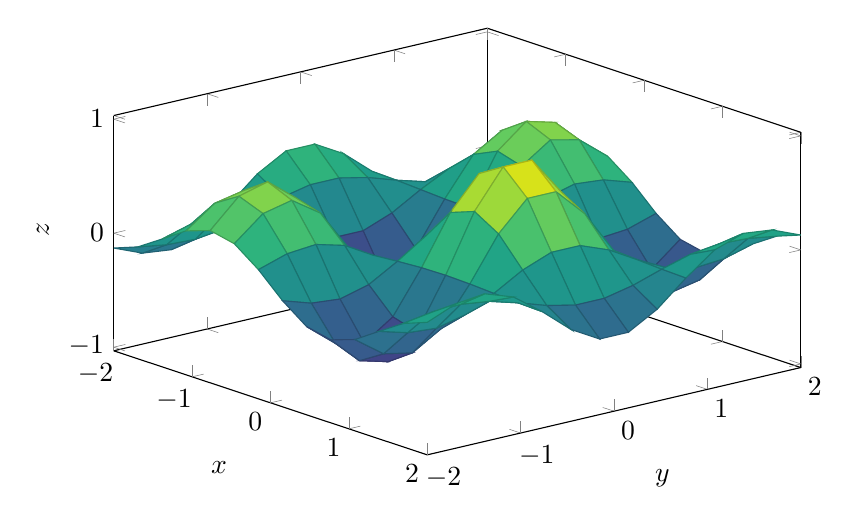
\begin{tikzpicture}\begin{axis}[width=0.85\linewidth,height=7cm,view={50}{30},colormap/viridis,xlabel=$x$,ylabel=$y$,zlabel=$z$]
\addplot3[surf,samples=14,domain=-2:2]{sin(deg(2*x))*cos(deg(2*y))*exp(-(x^2+y^2)/6)};
\end{axis}\end{tikzpicture}
\caption{Generated figure for \texttt{c8s1-f1} (parameters $a=2$, $b=6$).}\label{fig:c8s1-f1}
\end{figure}

\lipsum[101-102]

\subsection{Implementation notes}\label{sec:c8s1-i}
The core routine is shown in \cref{lst:c8s1}; its complexity is $\mathcal{O}(N\log N)$ per iteration~\cite{main-11}.

\begin{lstlisting}[language=python,caption={Reference implementation for c8s1.},label={lst:c8s1}]
import numpy as np

def step(u, dt, dx, D):
    """Explicit finite-difference update."""
    lap = (np.roll(u, 1) - 2 * u + np.roll(u, -1)) / dx**2
    return u + dt * D * lap

u = np.exp(-((np.linspace(0, 1, 200) - 0.5) ** 2) / 0.01)
for _ in range(1000):
    u = step(u, 1e-5, 1 / 200, 1.0)
\end{lstlisting}

\kant[1-12]
\begin{theorem}\label{thm:c8s1}
Let $A\in\mathbb{R}^{n\times n}$ be symmetric positive definite with condition number $\kappa$. Then the iteration converges and
$\lVert e_k\rVert_A \le 2\bigl(\tfrac{\sqrt\kappa-1}{\sqrt\kappa+1}\bigr)^k\lVert e_0\rVert_A$.
\end{theorem}
\begin{enumerate}[label=(\roman*)]
\item the bound in \cref{thm:c8s1} is sharp for some initial errors;
\item the constant $2$ cannot be improved in general;
\item preconditioning reduces the effective $\kappa$.
\end{enumerate}

\lipsum[60-60]
